
% Define which ratio you want to use 
%         43 to have a 4:3, 
%         169 to have 16:9.

\def\currentAspect{169}


% Uncomment the next line to define hasClickable if you want clickable figure
% \def\hasClickable{}

\documentclass[t,aspectratio=\currentAspect]{beamer}

% Header, packages
% ----------------
\def\oldAspect{43}
\def\newAspect{169}

\ifdefined\currentAspect
\else
\def\currentAspect{43}
\fi
\documentclass[t,aspectratio=\currentAspect]{beamer}

\usepackage{tcolorbox}
\RequirePackage[english]{babel}
\usepackage[linesnumbered,ruled,vlined]{algorithm2e}
\usepackage{mathrsfs,amsmath}
\usepackage{listings}
\usepackage{linehighlight}

\usepackage{pgfgantt}
\usepackage{pgfplots}
\usepackage{tikz}
\usetikzlibrary{intersections}
\usetikzlibrary{shapes}
\usetikzlibrary{chains}
\usetikzlibrary{arrows,positioning,calc}
\usetikzlibrary{decorations.markings}
\usetikzlibrary{patterns}
\usetikzlibrary{shapes.geometric}
\usetikzlibrary{matrix}
\usepackage[outline]{contour}
\usetikzlibrary{positioning}
\usetikzlibrary{trees}
\usetikzlibrary{patterns}
\usetikzlibrary{backgrounds}
\usetikzlibrary{arrows,shapes}
\usetikzlibrary{chains}
\usetikzlibrary{calc}
\usetikzlibrary{matrix}
\usetikzlibrary{decorations.pathreplacing}
\usetikzlibrary{decorations}
\usepackage{tikz-3dplot}
\usepgfplotslibrary{groupplots}
\usepackage{subfigure}
\ifdefined\hasClickable
\usepgfplotslibrary{clickable}
\fi
\usepackage{courier}
 
 
% Theme template 
% ---------------
\definecolor{c1}{rgb}{0,0.4470,0.7410}
\definecolor{c2}{rgb}{0.8500,0.3250,0.0980}
\definecolor{c3}{rgb}{0.9290,0.6940,0.1250}
\definecolor{c4}{rgb}{0.4940,0.1840,0.5560}
\definecolor{c5}{rgb}{0.4660,0.6740,0.1880}
\definecolor{c6}{rgb}{0.3010,0.7450,0.9330}
\definecolor{c7}{rgb}{0.6350,0.0780,0.1840}
\definecolor{c8}{rgb}{0,0.4325,0.1746}

\setbeamercolor{block title}{fg=c1,bg=white} % Colors of the block titles
\setbeamercolor{block body}{fg=black,bg=white} % Colors of the body of blocks
\setbeamercolor{block alerted title}{fg=white,bg=c1} % Colors of the highlighted block titles
\setbeamercolor{block alerted body}{fg=black,bg=c1!10} % Colors of the body of highlighted blocks
\setbeamercolor{frametitle}{fg=c1,bg=white} % Colors of the block titles

\setbeamersize{text margin left=5mm,text margin right=5mm} 
\setbeamertemplate{footline}[frame number]

\newtcolorbox{mybox}[1][]
{
  colframe = c1,
  sharpish corners,
  colback  = white
}

\setbeamertemplate{frametitle}{%
    \usebeamerfont{frametitle}\insertframetitle%
    \vphantom{g}% To avoid fluctuations per frame
    %\hrule% Uncomment to see desic2 effect, without a full-width hrule
    \par\hspace*{-\dimexpr0.5\paperwidth-0.5\textwidth}  \rule[0.5\baselineskip]{\paperwidth}{1.4pt}
    \par\vspace*{-\baselineskip}% <-- reduce vertical space after rule
}

\setbeamertemplate{itemize item}{\color{c1}$\blacktriangleright$}
\setbeamertemplate{itemize subitem}{\color{c2}$\blacktriangleright$}

\setbeamercolor{caption name}{fg=c1}

\newcommand{\argmin}{\operatornamewithlimits{arg\,min}}


%\setbeamertemplate{section in toc}[square unnumbered]
\setbeamercolor{section in toc}{fg=black}

\lstdefinelanguage
   [x64]{Assembler}     % add a "x64" dialect of Assembler
   [x86masm]{Assembler} % based on the "x86masm" dialect
   % with these extra keywords:
   {morekeywords={CDQE,CQO,CMPSQ,CMPXCHG16B,JRCXZ,LODSQ,MOVSXD, %
                  POPFQ,PUSHFQ,SCASQ,STOSQ,IRETQ,RDTSCP,SWAPGS, %
                  rax,rdx,rcx,rbx,rsi,rdi,rsp,rbp, vpxorq,   xor,  nopl,  vmovupsz ,  leal, vmovupsz, vcmppdz, vdivpdz, vmovupdz,%
                  r8,r8d,r8w,r8b,r9,r9d,r9w,r9b, %
                  r10,r10d,r10w,r10b,r11,r11d,r11w,r11b,zmm0,zmm1,zmm2,k1,k2, %
                  r12,r12d,r12w,r12b,r13,r13d,r13w,r13b, %
                  r14,r14d,r14w,r14b,r15,r15d,r15w,r15b}} % etc.


\definecolor{codehighlight}{rgb}{0.8500,0.3250,0.0980}
\definecolor{codebackground}{rgb}{1,1,1}

\newcommand{\gwidthd}{0.975\linewidth}
\newcommand{\gheightd}{0.6\linewidth}  
\newcommand{\gheightdd}{0.4\linewidth}  

\newcommand{\figurewidth}{0.9\linewidth}  
\newcommand{\figureheight}{0.85\textheight}  
\newcommand{\figureheightt}{0.7\linewidth}  

\newcommand{\Mod}[1]{\ (\mathrm{mod}\ #1)}




\ifdefined\hasClickable
\pgfplotsset{
    clickable coords = {(xy)}, % activates a snap-to-nearest feature
    annot/snap dist=20,
    /pgfplots/annot/js fillColor={["RGB",0,0.4470,0.7410]},
    /pgfplots/annot/point format/.initial={(\%.1f, \%.1f)},
    every semilogy axis/.append style={/pgfplots/annot/point format={(\%.1f,\%.1e)}},
    every semilogx axis/.append style={/pgfplots/annot/point format={(\%.1e,\%.1f)}},
    every loglog axis/.append style={/pgfplots/annot/point format={(\%.1e,\%.1e)}},
    %clickable coords size = {7,3}, % size in characters for the snapping pop ups
    %annot/popup size generic = {8,4}, % size in characters  for the rest
}
\fi

\AtBeginSection[]
{
   \begin{frame}[plain,noframenumbering]
        \frametitle{Table of contents}
        \tableofcontents[currentsection]
   \end{frame}
}

\beamertemplatenavigationsymbolsempty



% Add pie plots:

\makeatletter

\tikzstyle{chart}=[
    legend label/.style={font={\scriptsize},anchor=west,align=left},
    legend box/.style={rectangle, draw, minimum size=5pt},
    axis/.style={black,semithick,->},
    axis label/.style={anchor=east,font={\tiny}},
]

\tikzstyle{bar chart}=[
    chart,
    bar width/.code={
        \pgfmathparse{##1/2}
        \global\let\bar@w\pgfmathresult
    },
    bar/.style={very thick, draw=white},
    bar label/.style={font={\bf\small},anchor=north},
    bar value/.style={font={\footnotesize}},
    bar width=.75,
]

\tikzstyle{pie chart}=[
    chart,
    slice/.style={line cap=round, line join=round, very thick,draw=white},
    pie title/.style={font={\bf}},
    slice type/.style 2 args={
        ##1/.style={fill=##2},
        values of ##1/.style={}
    }
]

\pgfdeclarelayer{background}
\pgfdeclarelayer{foreground}
\pgfsetlayers{background,main,foreground}


\newcommand{\pie}[3][]{
    \begin{scope}[#1]
    \pgfmathsetmacro{\curA}{90}
    \pgfmathsetmacro{\r}{1}
    \def\c{(0,0)}
    \node[pie title] at (90:1.3) {#2};
    \foreach \v/\s in{#3}{
        \pgfmathsetmacro{\deltaA}{\v/100*360}
        \pgfmathsetmacro{\nextA}{\curA + \deltaA}
        \pgfmathsetmacro{\midA}{(\curA+\nextA)/2}

        \path[slice,\s] \c
            -- +(\curA:\r)
            arc (\curA:\nextA:\r)
            -- cycle;
        \pgfmathsetmacro{\d}{max((\deltaA * -(.5/50) + 1) , .5)}

        \begin{pgfonlayer}{foreground}
        \path \c -- node[pos=\d,pie values,values of \s]{$\v\%$} +(\midA:\r);
        \end{pgfonlayer}

        \global\let\curA\nextA
    }
    \end{scope}
}

\newcommand{\legend}[2][]{
    \begin{scope}[#1]
    \path
        \foreach \n/\s in {#2}
            {
                  ++(0,-10pt) node[\s,legend box] {} +(5pt,0) node[legend label] {\n}
            }
    ;
    \end{scope}
} 
 
 
\begin{document}
 
% Title Page
%-------------

\begin{frame}[plain,noframenumbering]

\vspace{10pt}

\begin{mybox}
\begin{center}
\parbox{.06\textwidth}{
\includegraphics[height=12pt]{logos/FNRS.eps}}
\parbox{.13\textwidth}{
\includegraphics[height=18pt]{logos/uLIEGE.eps}}
\parbox{.54\textwidth}{\centering \scriptsize Ensemble propagation for efficient uncertainty quantification of mechanical contact problems}
\parbox{.19\textwidth}{\hspace{20pt}
\includegraphics[height=12pt]{logos/sandia.eps}}
{ \tiny \underline{K. Liegeois}, R. Boman, E.~T. Phipps, M. Arnst}
\end{center}
\end{mybox}

\vspace{-10pt}
\begin{center}
\resizebox{1.\textwidth}{!}{%
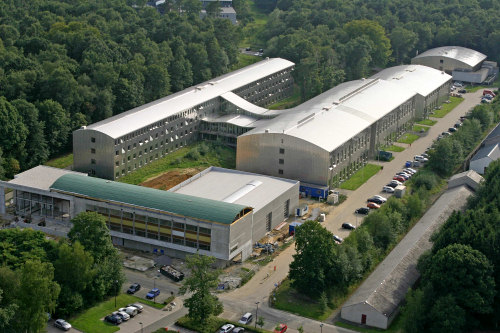
\includegraphics[height=5cm]{buildings/ulg.jpg}%
\quad
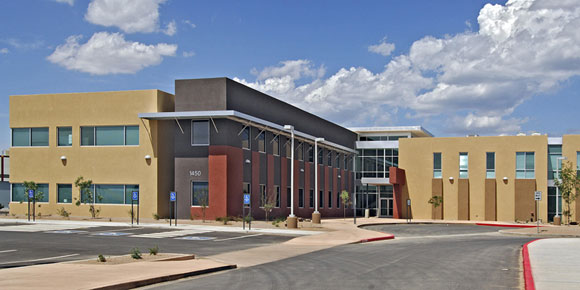
\includegraphics[height=5cm]{buildings/csri.jpg}%
}
\end{center}

\begin{center}
Weekly meeting,\\
\today.
\end{center}
\end{frame} 


% Slides
%-------------


% Example to show how to test whether the pdf is built with 4:3 or 16:9 ratio:
\ifx\currentAspect\oldAspect
	\def\sometext{The code has been built with the ratio for old screens 4:3}
\else
	\def\sometext{The code has been built with the ratio for new screens 16:9}
\fi



\begin{frame}{Slide }
\begin{itemize}
\setlength\itemsep{\fill}
\item \sometext,
\item Bullet 2,
\item Bullet 3,
\item Bullet 4.
\end{itemize}
\end{frame}


\begin{frame}{Tikz graph}
\begin{figure}[H]
\centering

\begin{tikzpicture}

\begin{axis}[
compat=1.3,
ymin=0, ymax=10,
width=\figurewidth,
height=\figureheight,
ylabel={Ylabel $y [\mathrm{m^2}]$},
xlabel={Xlabel $x [-]$},
xmin=0, xmax=40,
tick align=outside,
tick pos=left,
xmajorgrids,
x grid style={white},
ymajorgrids,
y grid style={white},
axis line style={white},
axis background/.style={fill=white!89.803921568627459!black},
legend pos=north west,
legend style={font=\small},
legend entries={plot 1,
   plot 2,
   plot 3
}
]

--(axis cs:2,54.61758)
--(axis cs:1,54.59319)
--cycle;

\addlegendimage{thick, c1, mark=*, mark size=2, mark options={solid}}
\addlegendimage{thick, c2, mark=*, mark size=2, mark options={solid}}
\addlegendimage{thick, c3, mark=*, mark size=2, mark options={solid}}

\addplot [thick, c1, mark=*, mark size=2, mark options={solid}, forget plot]
table {%
0 0
8 3
10 5
12 6
40 7
};
\addplot [thick, c2, mark=*, mark size=2, mark options={solid}, forget plot]
table {%
0 10
40 2
};
\addplot [thick, c3, mark=*, mark size=2, mark options={solid}, forget plot]
table {%
0 5
1 10
2 5
3 7
18 2
};
\end{axis}

\end{tikzpicture}
\vspace{-10pt}
\caption{Caption.}
\end{figure}
\end{frame}

\end{document}
